\documentclass{article}
\usepackage{pgf,tikz,tikzscale} 
\usepackage{amssymb}
\usepackage{tcolorbox}
\usepackage{xcolor}
\usepackage[utf8]{inputenc}
\usepackage[english]{babel}
\usepackage{multicol}
\usepackage{enumerate}	
\usepackage{graphicx,lipsum,pgfplots} 
\usepackage{amsmath, amsthm}                 
\usepackage[top=1in,bottom=1in, left=1in, right=1in] {geometry}  
\usepackage{fancyhdr}       
\usepackage{blkarray}


\pagestyle{fancy}              
\lhead{Math 5563 \newline Graph Theory HW1}   
\rhead{Warren Keil}







\begin{document}
\setlength{\parindent}{0cm}   %%%%%%%% KEEP THIS  for block style paragraphs. 



%%%%%%%%%%%%%%%%%        1a   %%%%%%%%%%%%%%%%%%%%
\textbf{1.} Create a graph with 5 vertices and 7 edges. Label the vertices A, B, C, D, and E. Does this graph contain an Euler path? If so, indicate what the path is. If not, explain why the graph doesn't have an
Euler path. Does the graph have an Euler circuit? If so, indicate what the circuit is. If not, explain
why the graph doesn't have an Euler circuit.
\vspace{3mm}

\textbf{Solution.} Let \( G = (V,E) \ni V=\{ A,B,C,D,E\}, E=\{AB,AC,AD,AE,BC,CD,DE\} \). Then \(G\) does contain an Euler path. An Euler path of \(G\) is \(P = D,E,A,D,C,A,B,C \). We notice we had to begin and end on the vertices that possess an odd degree. Next, we notice that \(G\) does not have an Euler circuit. This is known by Euler's First Theorem which states that a graph is connect and all of its vertices have an even degree if and only if that graph has at least one Euler circuit. Since our graph \(G\) is connect but does not have an even degree for each of its vertices then it cannot have at least one Euler circuit. 



\vspace{1mm}
\begin{center}
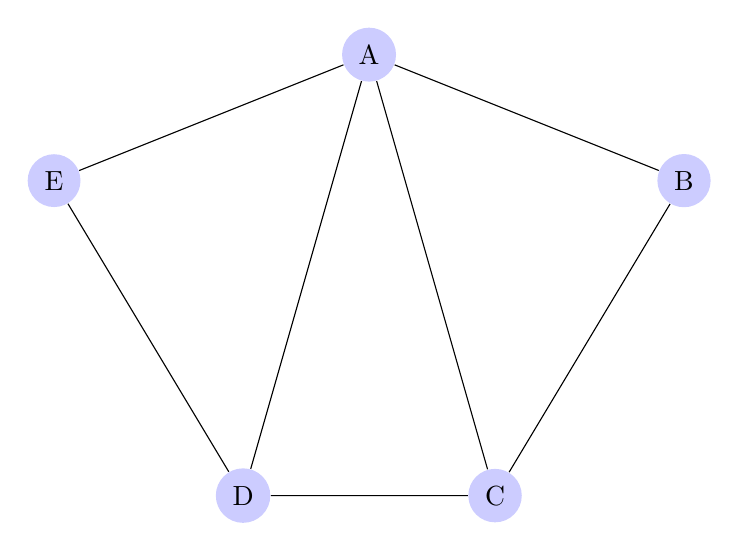
\begin{tikzpicture}
  [scale=.8,auto=left,every node/.style={circle,fill=blue!20}]
  \node (a) at (5,10) {A};
  \node (b) at (10,8)  {B};
  \node (c) at (7,3)  {C};
  \node (d) at (3,3) {D};
  \node (e) at (0,8)  {E};

  \foreach \from/\to in {a/b, b/c, c/d, d/e, a/e,a/c,a/d}
    \draw (\from) -- (\to);

\end{tikzpicture}
\end{center}

\textbf{2.} If your graph in (1) is not an Euler circuit, add or subtract edges so that it is an Euler circuit. Clearly indicate the added or subtracted edges.

\vspace{2mm}
\textbf{Solution.} To create an Euler circuit, we first remove the edges \(AD \) and \(AC\) from our graph \(G\). Now, our cycle is \(C= D,E,A,B,C\). 

\begin{center}
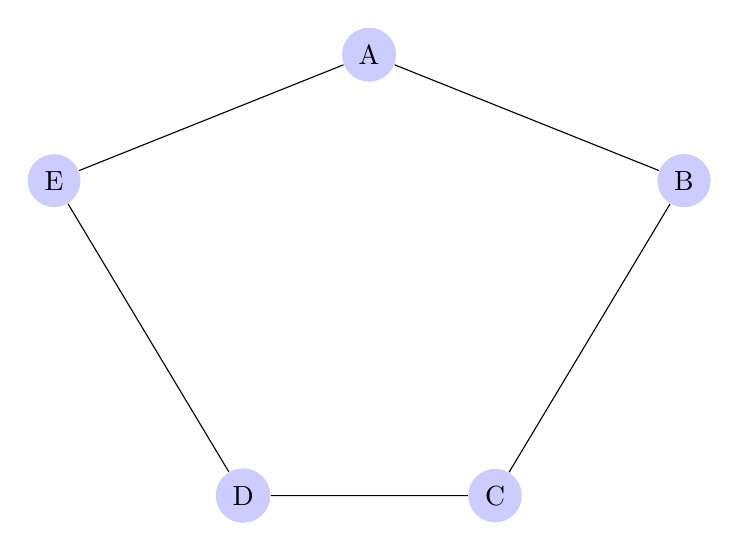
\begin{tikzpicture}
  [scale=.8,auto=left,every node/.style={circle,fill=blue!20}]
  \node (a) at (5,10) {A};
  \node (b) at (10,8)  {B};
  \node (c) at (7,3)  {C};
  \node (d) at (3,3) {D};
  \node (e) at (0,8)  {E};

  \foreach \from/\to in {a/b, b/c, c/d, d/e, a/e}
    \draw (\from) -- (\to);

\end{tikzpicture}
\end{center}

\newpage
\textbf{3.}  Create a Hamiltonian path using 5 vertices and at least 4 edges. Label the vertices A, B, C, D, and E. Clearly indicate what the path is.

\vspace{2mm}
\textbf{Solution.} Let \(G= (V,E)\) where \( V=\{A,B,C,D,E\}, E=\{AB, BC, CD, DE\}\). Let the path be \(P= ~ A,B,C,D,E\). 
\begin{center}
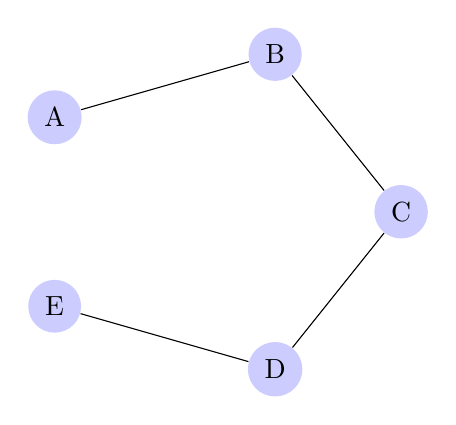
\begin{tikzpicture}
  [scale=.4,auto=left,every node/.style={circle,fill=blue!20}]
  \node (a) at (0,8) {A};
  \node (b) at (7,10)  {B};
  \node (c) at (11,5)  {C};
  \node (d) at (7,0) {D};
  \node (e) at (0,2)  {E};

  \foreach \from/\to in {a/b, b/c, c/d,d/e}
    \draw (\from) -- (\to);

\end{tikzpicture}
\end{center}



\vspace{4mm}
\textbf{4.} What is the maximum number of edges you can use in order to still have a Hamiltonian path (if you have 5 vertices)?

\vspace{2mm}
\textbf{Solution.} The maximum number of edges you can use to have a Hamiltonian path on a graph of \(n\) vertices are \(n-1\) edges. So the maximum number of edges that our graph of five vertices can have and still have a Hamilton path is four edges. 



\vspace{4mm}
\textbf{5.} What will the degrees of the vertices have to be in order to have a single graph (with n vertices) which is an Euler path, Euler circuit, Hamiltonian path, and Hamiltonian circuit? (Hint: Consider a theorem
that was presented in class and experiment with some small graphs.)

\vspace{2mm}
\textbf{Solution.} Let \(G\) be a graph with \(n\) vertices such that \(G\) has an Euler path, Euler circuit, and a Hamilton circuit. Since \(G\) has an Euler path, then by the Euler path theorem, we know that \(G\) either has zero or two vertices with an odd degree. And since \(G\) has an Euler circuit, then by Euler's First Theorem, we know that the degree of every vertex of \(G\) must be even. Combing these two properties of \(G\) we see that \(G\) cannot have any vertices with odd degree. And lastly, since \(G\) contains a Hamilton circuit, then the degree of each vertex must equal two.  


\vspace{2mm}
Putting these facts together we see that the graph \(G\) will have a degree sequence of
\[
 d(G) =\underbrace{(2,2, \ldots, 2)}_{\text{\(n\) times}}.
\]
\begin{flushright}
\qed
\end{flushright}











\end{document}
